\section{Integrazione}
\label{integrazione}

L'analisi esplorativa dei due datasets, anche in vista dell'applicazione dei metodi di Machine Learning, ha prodotto come risultato due nuovi datasets composti da un insieme ridotto di attributi, ritenuti rilevanti e non ridondanti per lo studio e gli obiettivi prefissati. Il numero di record è rimasto inalterato.
\par
L'integrazione dei due nuovi datasets ha avuto luogo in due passi separati. Inizialmente, è stata utilizzata una componente \textit{tMap} per associare al dataset dei tiri le statistiche degli attaccanti. Dopodiché, questo dataset consistente dei nuovi attributi è stato utilizzato assieme al dataset delle statistiche per associare, con un'altra componente \textit{tMap}, le informazioni relative al difensore.
\par
\begin{figure}[H]
\caption{Pipeline d'integrazione dati implementata con \textit{Talend Studio}}
	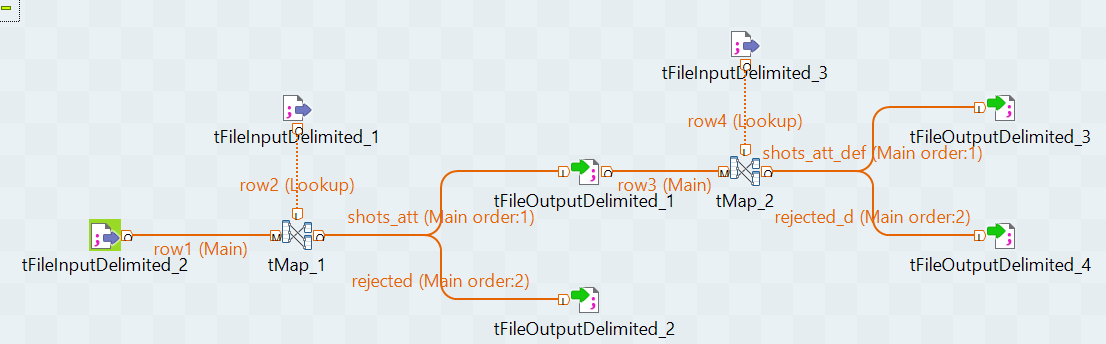
\includegraphics[width=\linewidth]{pipeline_talend1.png}
\end{figure}

Non utilizzando un ID univoco che identifica un giocatore per effettuare l'integrazione tra i due datasets ma i nomi stessi degli atleti, abbiamo optato per l'utilizzo della stessa funzione descritta nella \autoref{preparazione}, così da uniformare i nomi presenti (scritti in minuscolo ordinati lessicograficamente) nei due datasets. 
\par

Effettuata l'integrazione, per verificare la consistenza del matching in ciascuno dei due passi è stato creato un file denominato \textit{rejected} in cui sono state inserite le istanze respinte, non trovando una corrispondenza perfetta.
\par
Circa una decina di nomi sono risultati in questa lista: sono risolti manualmente nella routine \texttt{EditShotLogs\_0.1.java}\autoref{matchNamesr}, eseguita in pipeline da Talend, poichè sarebbe stato problematico e dispendioso usare funzioni di edit distance appositamente parametrizzate per così pochi e particolari casi.

\begin{code}
\captionof{listing}{Metodo matchNames da EditShotLogs\_0.1.java}
\label{matchNamesr}
\begin{minted}{java}
public static String matchNames(String name1) {
	String[] def = {"Barea, Jose Juan", "Hardaway Jr., Tim", 
		"Aminu, Al-Farouq", "Nene", "Mbah a Moute, Luc",
		"Hayes, Charles", "Lucas III, John", "Taylor, Jeff",
		"Rice Jr., Glen", "Datome, Gigi", "McAdoo, James Michael"};
	String[] stats = {"J.J. Barea", "Tim Hardaway", 
		"Al-Farouq Aminu", "Nene Hilario", "Luc Mbah",
		"Chuck Hayes", "John Lucas", "Jeffery Taylor",
		"Glen Rice", "Luigi Datome", "James Michael"};
	String[] results = {"barea jj", "hardaway tim", 
		"al-farouq aminu", "nene hilario", "luc mbah",
		"chuck hayes", "john lucas", "jeffery taylor",
		"glen rice", "datome luigi", "james mcadoo michael"};
	if (Arrays.asList(def).contains(name1) || 
		Arrays.asList(stats).contains(name1)) {
		for (int i = 0; i < def.length; i++) {
			if (name1.equals(def[i]) || 
				name1.equals(stats[i])) {
				return results[i];
			}
		}  
	}
	String[] names1 = name1.replaceAll("[^a-zA-Z ]", "")
		.toLowerCase().split("\\s+");
	Arrays.sort(names1);
	String nuova = "";
	for (int i = 0; i < names1.length; i++) {
		nuova += names1[i];
		nuova += " ";
	}
	nuova = nuova.trim();
	return nuova;
}
\end{minted}
\end{code}

\subsection{Misure di qualità del dataset integrato}

\subsubsection{Currency, Volatility e Timeliness}
Un aspetto importante dei dati coinvolti nel nostro processo di integrazione è il loro cambiamento nel tempo. I database a nostra disposizione contemplano l'anno di campionato 2014-2015.

\textit{Currency}, definita come la velocità degli aggiornamenti \cite{batini2006}, è calcolabile con la seguente formula\cite{doi:10.1287/mnsc.44.4.462}
\begin{equation}
Currency = Age + (DeliveryTime - InputTime)
\end{equation}
\textit{Age} misura l'età dei dati quando vengono ricevuti, \textit{DeliveryTime} è l'istante in cui il prodotto che utilizza queste informazioni è consegnato all'utente finale mentre \textit{InputTime} è l'istante in cui il dato è stato effettivamente ottenuto.
Il termine $(DeliveryTime - InputTime)$ misura quindi il periodo di tempo che trascore prima che il prodotto che utilizza i nostri dati sia pronto ed effettivamente utilizzabile.

Poichè l'anno corrente è 2019, i dati hanno una \textit{Age} di 4 anni. $(DeliveryTime - InputTime)$ risulta quindi trascurabile e \textit{Currency} è equivalente  ad \textit{Age}.

Supponendo inoltre che le statistiche dell'NBA rimangano rilevanti per le 3 stagioni successive, la \textit{volatilità} dei dati è uguale a 3 anni.

\textit{Timeliness}, calcolata con 

\begin{equation}
\max\{{0, 1 - \frac{Currency}{Volatility}}\}
\end{equation}

Vale quindi 0, rappresentando una cattiva tempestività del nostro dataset.

\subsubsection{Completability}

\begin{figure}[H]
\caption{Rappresentazione grafica della completabilità \cite{batini2006}}
\label{completabilitypic_gen}
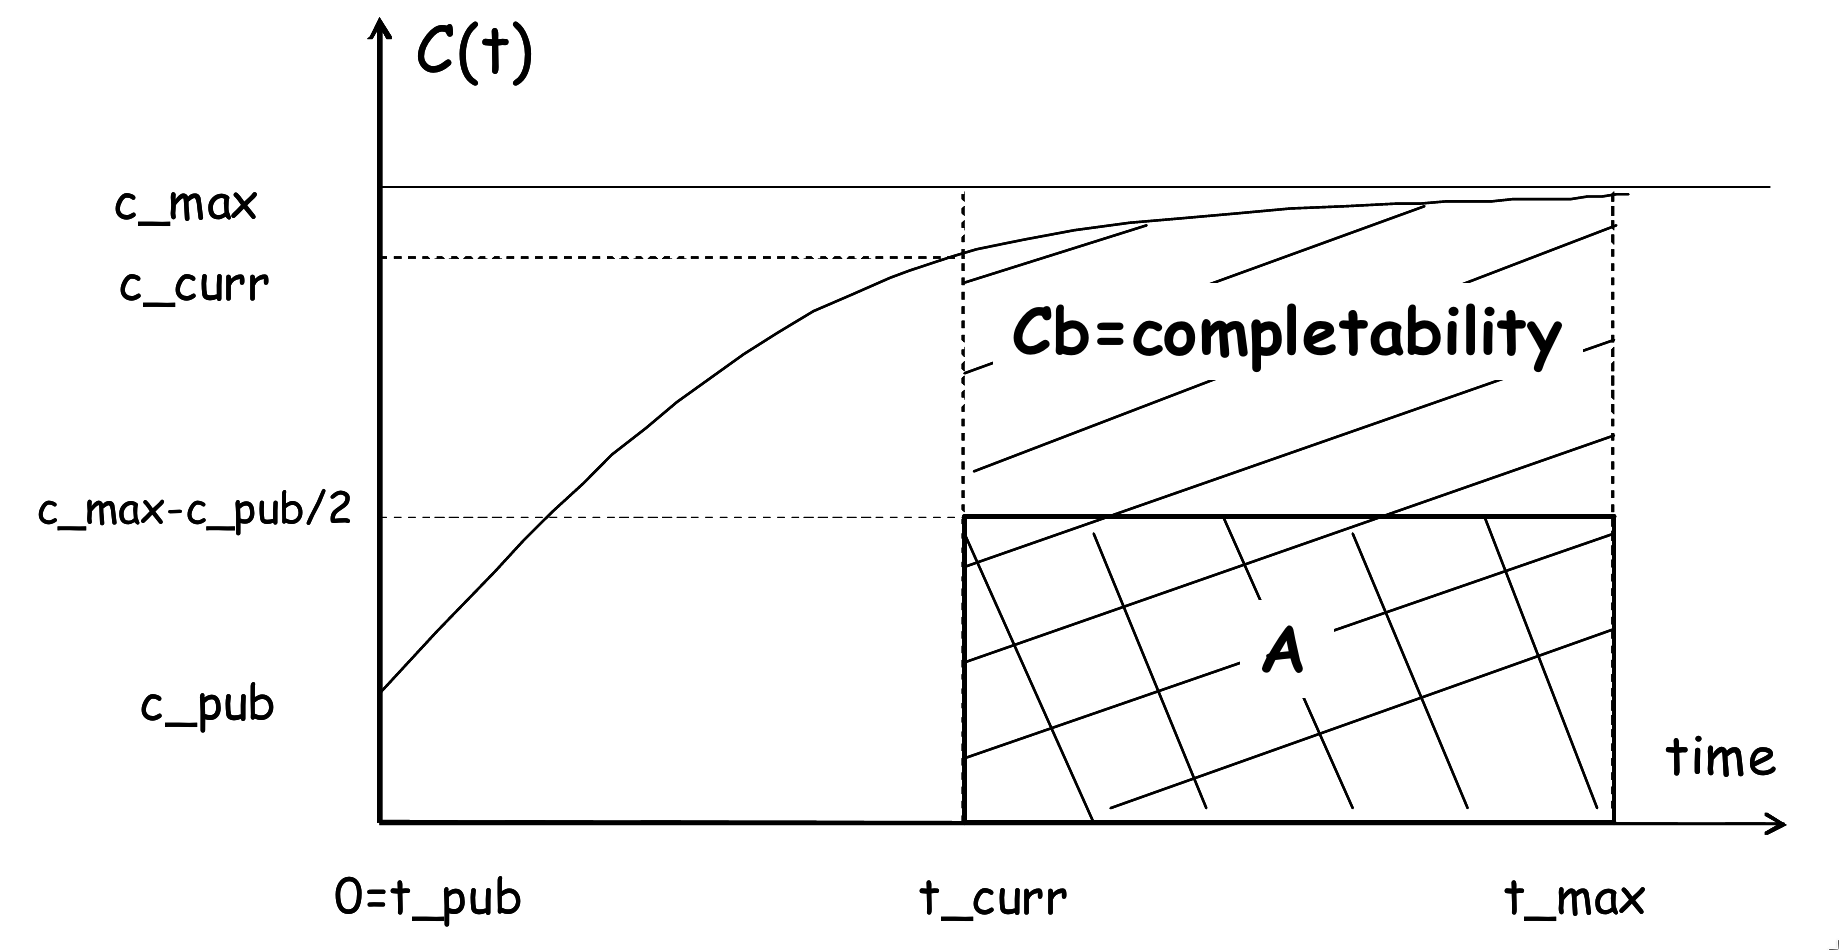
\includegraphics[width=\linewidth]{completability_gen.png}
\end{figure}

Essendo i nostri dataset originari di servizi Web e riflettendo eventi reali distribuiti durante l'anno, ne vengono costantemente pubblicate versioni aggiornate.

La \textit{Completabilità} è un'interessante metrica che ci permette di visualizzare la dinamica di evoluzione temporale della completezza.

Consideriamo una funzione $C(t)$, definita come il valore della completezza all'istante t, con $t \in [t_{pub}, t_{max}]$, dove $t_{pub}$ è l'istante iniziale di pubblicazione dei dati e $t_{max}$ il tempo massimo in cui verrà completato l'ultimo degli aggiornamenti dei dati previsiti.

La \textit{completabilità} dei dati è quindi definibile come \cite{batini2006}:

\begin{equation}
\int_{t_{curr}}^{t_{max}} C(t)
\end{equation}

Con $t_{curr}$ l'instante in cui essa viene calcolata ($t_{curr} < t_{max}$).

La \autoref{completabilitypic_gen} generalizza come si presenta, dove $c_{i}$ valore di completezza stimato per un generico $t_{i}$.


La Completabilità è definita dall'area segnata come \textit{Cb}. Il confronto con $A$, definita dalla \autoref{completability_a} permette di definire gli intervalli $[Alto, Media, Bassa]$ per la completabilità.
\begin{equation}
\label{completability_a}
A = (t_{max} - t_{curr}) * \frac{c_{max} - c_{pub}}{2}
\end{equation}



\par

Per dare un'idea di che completabilità esibiscono i dataset che consideriamo supponiamo che il ritardo con cui otteniamo i dati sulle partite appena avvenute sia trascurabile, i.e. ad un istante $t$ si abbiano i dati delle partite fino a $t-1$.
\par
	% TODO: DECIDERE SE USARE %
	Stimiamo la completezza percentuale dei dati, in un istante \textit{t}, con 
	\begin{equation}
	C(t) = \frac{\sum\limits_{y=c-p-1}^{c-1} M_{y} + m_{c,t}}{\sum\limits_{y=c-p-1}^{c} M_{y}} \times 100
	\end{equation}
	Dove \begin{itemize}
		\item $M_y$ è il numero totale di partite nella stagione $y$;
		\item $m_{c,t}$ il numero totale di partite nella stagione $y$ fino all'istante $t$;
		\item $c$ la stagione considerata
		\item $p$ numero di stagioni precedenti a quella che si vuole considerare che si suppongono rilevanti e parte del dataset.
	\end{itemize}

Considerando tutti gli istanti $t$ in cui siano giocate delle partite, ottenute da \cite{nba_schedule} e utilizzando $y = 2019, c = 3$ (considerando quindi i dati delle stagioni 2019, 2018, 2017, 2016, con 2019 stagione oggetto del dataset), la completabilità evolve secondo la \autoref{completabilitypic} attestandosi su un valore medio.

Scegliendo una finestra temporale più estesa la completabilità mostra un andamento periodico.

Infatti da inizio stagione (Ottobre) fino alla sua fine (Maggio) continuano ad essere forniti dati nuovi dopo ogni singola partita; nel periodo da Maggio a Ottobre invece non ci sono partite e nessun nuovo dato viene generato; infine ad Ottobre inizia un nuovo campionato, rendendo obsoleti i dati più vecchi della finestra mentre si abbassa la completezza.


% TODO: Aggiungere C(t) sull'asse Y, sostituire Date con Time nell'asse X.
\begin{figure}
\caption{Rappresentazione grafica della completabilità nel nostro esempio}
\label{completabilitypic}
\includegraphics[width=\linewidth]{completability}
\end{figure}